\section{Results}

We now present our results, focusing in particular on whether NLI benchmarks provide a discriminative signal for fully trained out models (\cref{subsec:fully_trained}), how their performance develops during training (\cref{subsec:during_training}), and what is the impact of evaluation data contamination (\cref{subsec:contamination}). 
Next, we investigate whether there is still room for improvement (\cref{subsec:saturation}) and how model judgements compare to human judgements for ambiguous or vague questions (\cref{subsec:chaosnli_dist}).

\subsection{Informativeness for fully trained models}\label{subsec:fully_trained}

\begin{figure*}[t]
    \begin{subfigure}[b]{\textwidth}
        \hspace{5mm}
        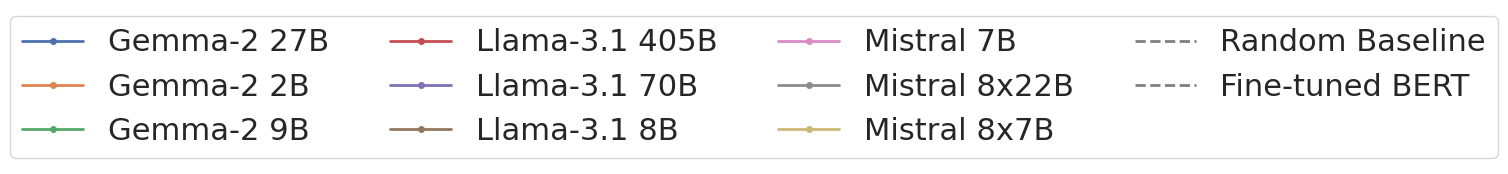
\includegraphics[width=0.95\textwidth]{figures/legend}
        \vspace{-3mm}
    \end{subfigure}\\
    \begin{subfigure}[b]{0.217\textwidth}
    \centering
    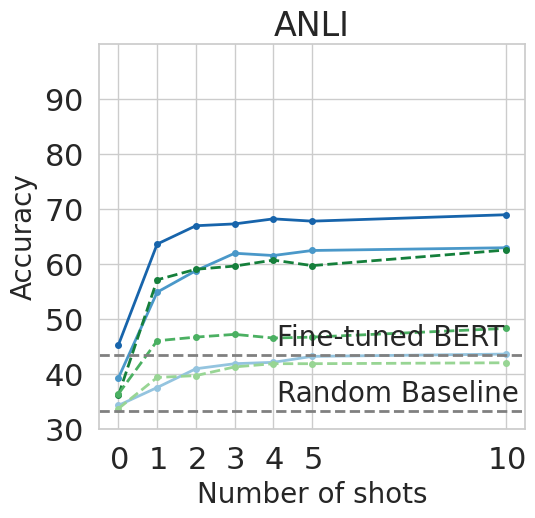
\includegraphics[height=3.45cm]{figures/anli}
    \caption{ANLI}
    \end{subfigure}
    \label{fig:anli}
    \begin{subfigure}[b]{0.19\textwidth}
    \centering
    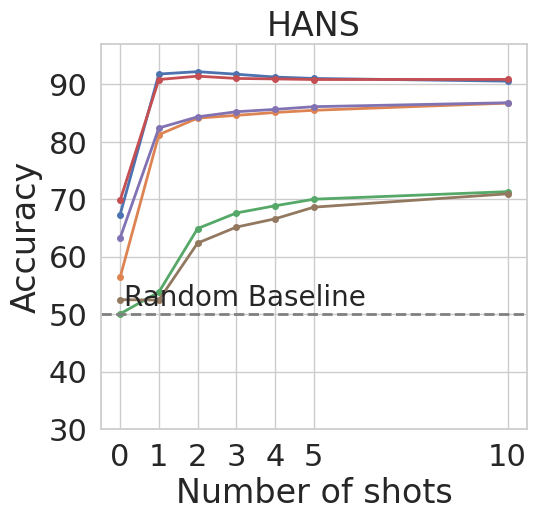
\includegraphics[height=3.45cm, trim=25mm 0 0 0, clip]{figures/hansnli}
    \caption{HANS}
    \label{fig:hans}
    \end{subfigure}
    \begin{subfigure}[b]{0.19\textwidth}
    \centering
    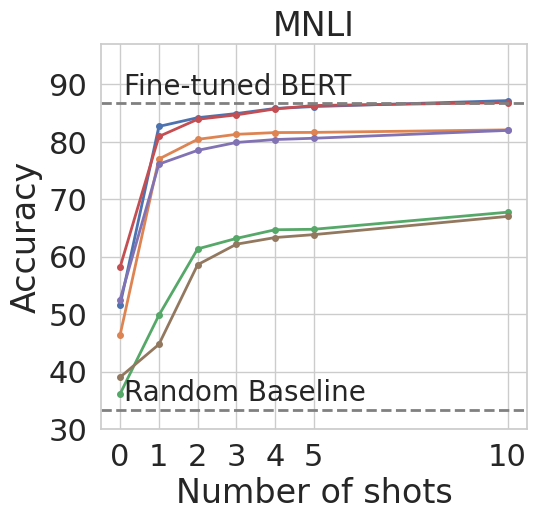
\includegraphics[height=3.45cm, trim=25mm 0 0 0, clip]{figures/mnli_matched}
    \caption{MNLI}
    \label{fig:mnli}
    \end{subfigure}
    \begin{subfigure}[b]{0.19\textwidth}
    \centering
    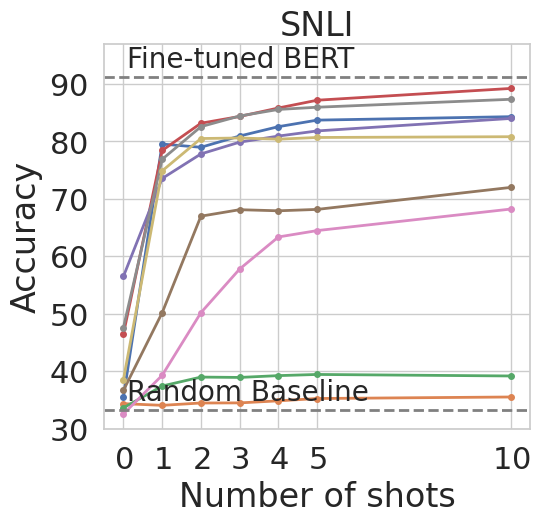
\includegraphics[height=3.45cm, trim=25mm 0 0 0, clip]{figures/snli}
    \caption{SNLI}
    \label{fig:snli}
    \end{subfigure}
    \begin{subfigure}[b]{0.19\textwidth}
    \centering
    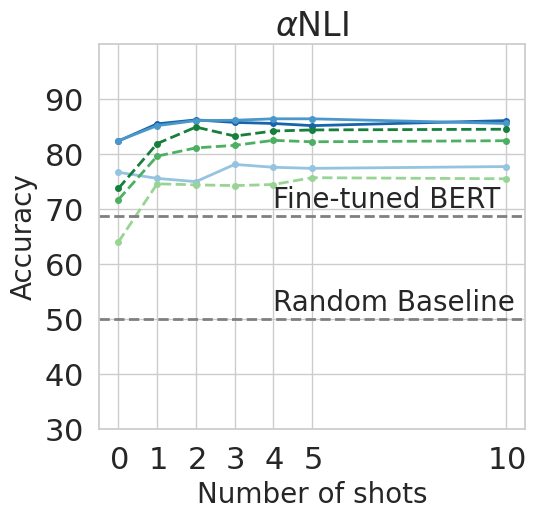
\includegraphics[height=3.45cm, trim=25mm 0 0 0, clip]{figures/abductivenli}
    \caption{$\alpha$NLI}
    \label{fig:alphanli}
    \end{subfigure}
    \caption{\textbf{Performance across shots.} We show the accuracies for six fully pre-trained models on the five NLI benchmarks. Dashed lines indicate random and finetuned-BERT baselines.}\label{fig:shot_performance}
\end{figure*}

To get an overall estimate of the difficulty of NLI and the extent to which it can discriminate models, we first consider the performance of fully pre-trained models from the respective model series.

\paragraph{Accuracy across shots}
For each of the models, we compute results with a variable number of shots.\footnote{For each number of few-shot examples, samples were chosen randomly from the dev or train set once and kept fixed throughout the experiments.}
We report the results in \cref{fig:shot_performance}, along with a chance baseline and the results of a fine-tuned BERT model.
For all models, we observe rather poor zero-shot performance for all tasks, except $\alpha$NLI, confirming previously reported results by \citet{ohmer2024form}, \citet{weber-etal-2023-mind}, and \citet{dutt-etal-2024-investigating}.
When more few-shot examples are added, performance starkly improves.
Even with just one in-context example, the performance is significantly better than the zero shot accuracy.
Adding more than three or four examples marginally improves performance and saturates around ten few-shot examples. 
Among the five benchmarks, the most challenging benchmark is ANLI.
Although the larger models in the Llama and Mistral series far outperform the finetuned BERT baseline, they do not exceed 70\% accuracy -- to some extent confirming the difficulty of the benchmark reported by \citet{brown2020language}.

\paragraph{Model discriminability}
For discriminability, virtually all benchmarks provide a clear gap between the smaller and larger models for both families of models.
For example, for the Llama series, 405B performs the best followed by the 70B and then the 8B model.
Though these three models are trained on the same amount of text tokens, performance clearly improves with scale.
The exception to this pattern is $\alpha$NLI, which appears to be near-saturated already at 70B with an accuracy of around 85\%.
We conclude from these results, that the benchmarks provide a useful signal to compare trained-out models, though it is unclear to what extent their performance has saturated, which we discuss in more detail in \cref{subsec:saturation}.

\subsection{Informativeness during training}\label{subsec:during_training}

Next, we investigate if NLI datasets provide a good signal during training.
To this end, we pre-train Llama-3 architecture-based 8B and 70B models from scratch for 2T tokens. The details of the pre-training setup are provided in \cref{appx:experiments}.

\paragraph{Training curves}
In \cref{fig:performance_training}, we show how four-shot performance develops during training.
We see that for most benchmarks, the 8B and 70B model quickly start to diverge.
The 70B model starts improving after 250B tokens for ANLI and $\alpha$NLI; it crosses fine-tuned BERT performance after 500B tokens.
On the other hand, the development of performance for the 8B model is slow, not exceeding chance accuracy for HANS, MNLI, and SNLI.
From the final model performance of 8B depicted in \cref{fig:shot_performance}, we can conclude that the 8B model improves fairly late in pre-training.
We did not have the budget for a full pre-training run, but longer training seems to help for NLI tasks, further supporting the claim that NLI models can provide a useful signal.

\begin{figure*}[t]
    \begin{subfigure}[b]{0.20\textwidth}
    \centering
    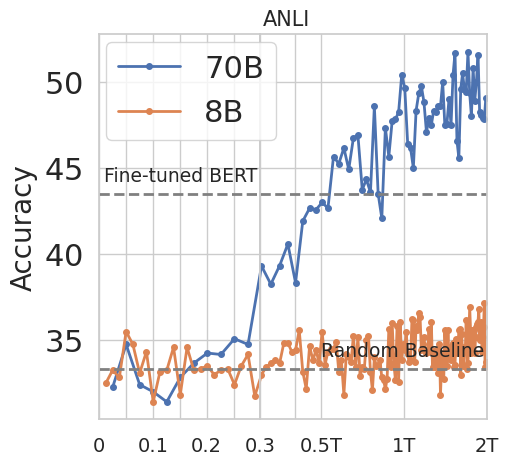
\includegraphics[height=3.2cm]{figures/anli_intermediate}
    \caption{ANLI}
    \end{subfigure}
    \label{fig:anli_int}
    \begin{subfigure}[b]{0.19\textwidth}
    \centering
    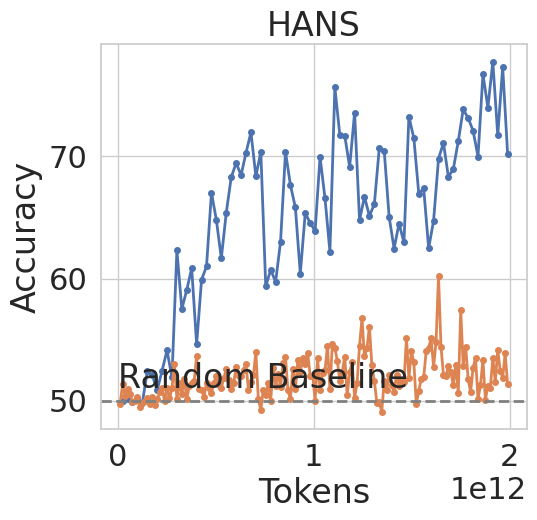
\includegraphics[height=3.2cm, trim=11mm 0 0 0, clip]{figures/hansnli_intermediate}
    \caption{HANS}
    \label{fig:hans_int}
    \end{subfigure}
    \begin{subfigure}[b]{0.19\textwidth}
    \centering
    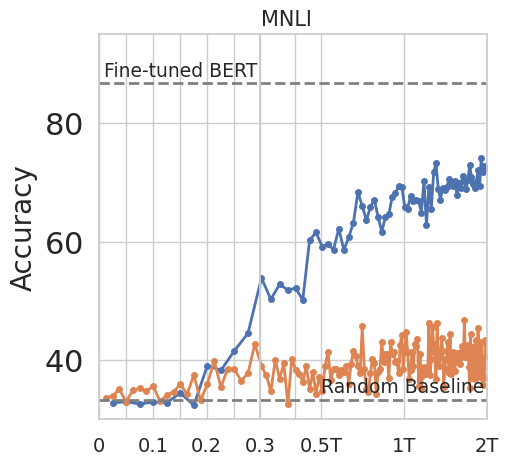
\includegraphics[height=3.2cm, trim=11mm 0 0 0, clip]{figures/mnli_matched_intermediate}
    \caption{MNLI}
    \label{fig:mnli_int}
    \end{subfigure}
    \begin{subfigure}[b]{0.19\textwidth}
    \centering
    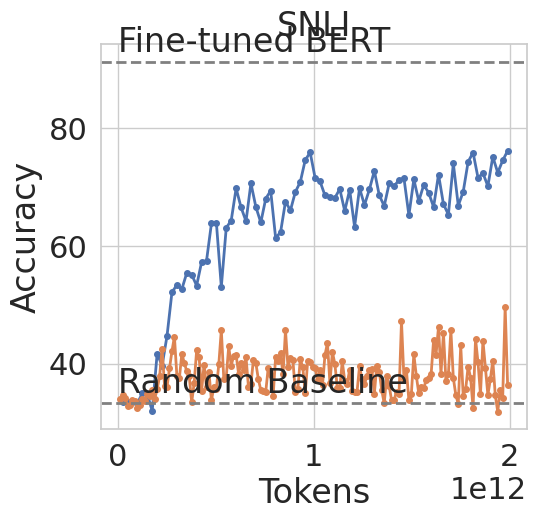
\includegraphics[height=3.2cm, trim=11mm 0 0 0, clip]{figures/snli_intermediate}
    \caption{SNLI}
    \label{fig:snli_int}
    \end{subfigure}
    \begin{subfigure}[b]{0.19\textwidth}
    \centering
    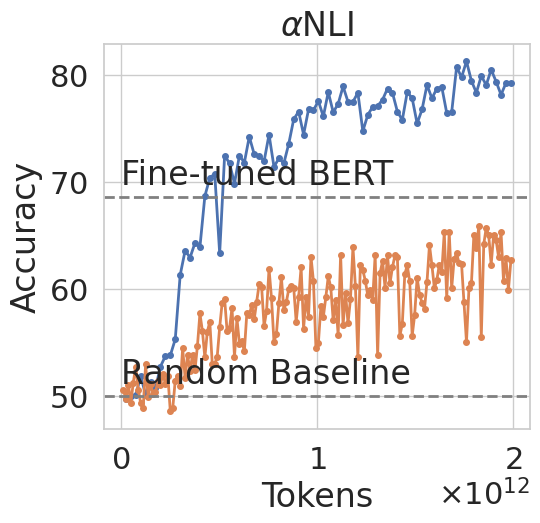
\includegraphics[height=3.2cm, trim=11mm 0 0 0, clip]{figures/abductivenli_intermediate}
    \caption{$\alpha$NLI}
    \label{fig:alphanli_int}
    \end{subfigure}
    \caption{\textbf{Performance during pre-training}. 
    We show how accuracy for the five benchmarks develops during pre-training for two Llama-3 style models.}\label{fig:performance_training}
\end{figure*}

\begin{table}
\centering
\resizebox{0.45\textwidth}{!}{
\begin{tabular}{lcccc}
    & \multicolumn{2}{c}{8B} & \multicolumn{2}{c}{70B} \\
    & $mon_{Acc}$  & $mon_{NLL}$ & $mon_{Acc}$ & $mon_{NLL}$ \\
    \toprule
    $\alpha$NLI & 0.62 & 0.62 & 0.79 & 0.79 \\
    \midrule
    ANLI & - & - & 0.67 & 0.47 \\
    \midrule
    HANS & 0.32 & 0.46 & 0.57 & 0.63 \\
    \midrule
    MNLI & 0.34 & 0.51 & 0.77 & 0.80 \\
    \midrule
    SNLI & 0.05 & 0.38 & 0.64 & 0.65 \\
    \bottomrule
    \end{tabular}
}
    \caption{\textbf{Monotonicity values during the course of training.} We report monotonicity both for accuracy ($mon_{Acc}$) and negative log likelihood of the correct answer ($mon_{NLL}$).}
\label{tab:monotonicity}
\end{table}

\paragraph{Utility for ablations}
A requirement for a benchmark to provide a useful signal during training is that it develops relatively monotonically during training.
The plots in \cref{fig:performance_training} suggest that this is not the case for most of the benchmarks for the 8B model.
Following \citet{variancepaper}, we quantify the benchmarks' monotonicity -- defined as the rank correlation (Kendall Tau) between a monotonically increasing array and the array containing the benchmark scores during training -- on both a discrete (accuracy) and continuous metric (NLL). 
In \cref{tab:monotonicity}, we can see that, despite the benchmarks' moderate sizes, monotonicity is low for accuracy as well as NLL, suggesting that the benchmark may not be suitable for monitoring performance on closely-spaced checkpoints at this scale. 

\subsection{Contamination analysis}\label{subsec:contamination}

Now that we have concluded that NLI benchmarks provide a signal both for final models and during pre-training, we analyse the extent to which scores may be driven by evaluation data contamination.
Using the methodology of \citet{singh2024evaluationdatacontaminationllms} and \citet{dubey2024llama}, we analyse contamination by assigning a score to each evaluation sample which represents the percentage of tokens in the sample that is part of an 8-gram occurring in the pre-training datamix.
Following \citet{singh2024evaluationdatacontaminationllms}, we select contamination thresholds using \texttt{ConTAM}, considering the estimated performance gain (EPG) for each threshold, which is defined as the difference in performance score on the full evaluation set and the `uncontaminated' set.\footnote{A threshold of 0 implies that all examples with non-zero contamination scores to be marked as contaminated, as we increase the threshold, examples are moved to the `uncontaminated' subset.}
Since EPG is model-dependent, we use the 8B and 70B models we trained from scratch to observe the effect of contamination. 

\begin{figure*}[t]
    \begin{subfigure}[b]{0.20\textwidth}
    \centering
    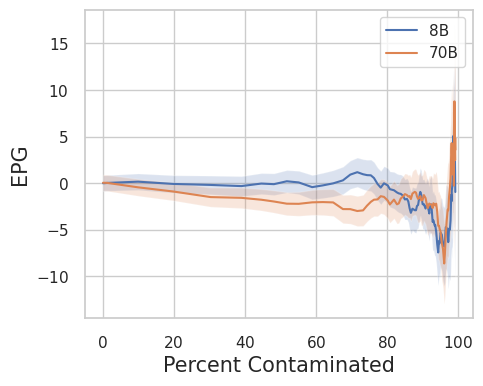
\includegraphics[height=2.6cm]{figures/contamination_anli}
    \caption{ANLI}
    \end{subfigure}
    \label{fig:cont_anli}
    \begin{subfigure}[b]{0.19\textwidth}
    \centering
    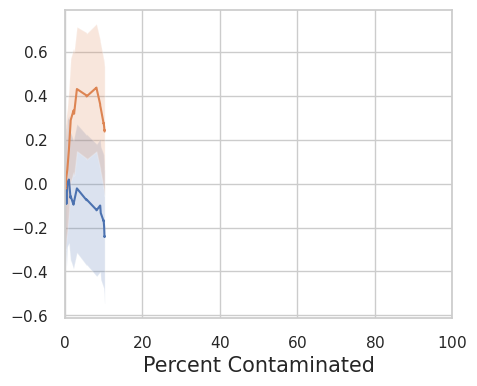
\includegraphics[height=2.6cm]{figures/contamination_hansnli}
    \caption{HANS}
    \label{fig:cont_hans}
    \end{subfigure}
    \begin{subfigure}[b]{0.19\textwidth}
    \centering
    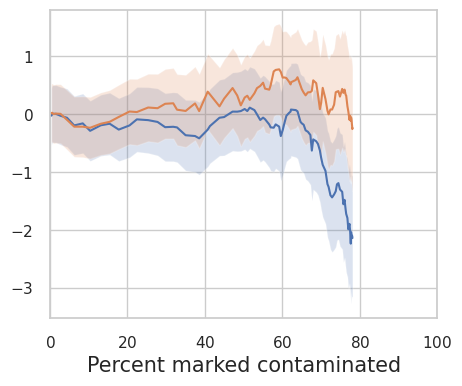
\includegraphics[height=2.6cm]{figures/contamination_mnli_matched}
    \caption{MNLI}
    \label{fig:cont_mnli}
    \end{subfigure}
    \begin{subfigure}[b]{0.19\textwidth}
    \centering
    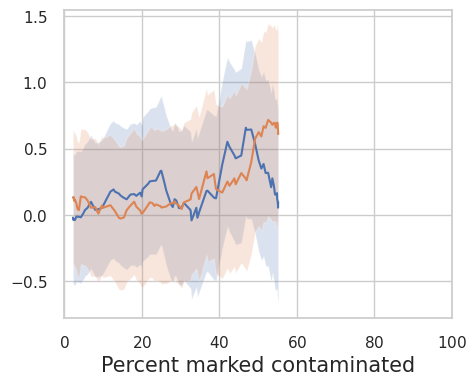
\includegraphics[height=2.6cm]{figures/contamination_snli}
    \caption{SNLI}
    \label{fig:cont_snli}
    \end{subfigure}
    \begin{subfigure}[b]{0.19\textwidth}
    \centering
    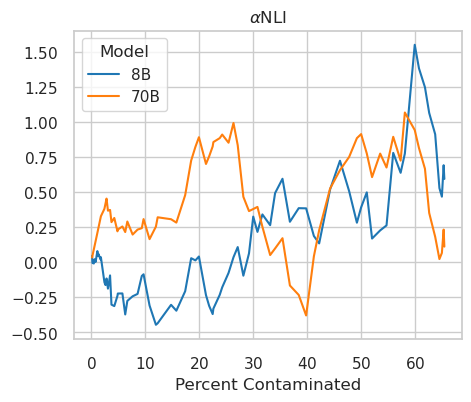
\includegraphics[height=2.6cm]{figures/contamination_abductivenli}
    \caption{$\alpha$NLI}
    \label{fig:cont_alphanli}
    \end{subfigure}
    \caption{\textbf{Contamination results.} We show the EPG vs the percent of the evaluation dataset marked as contaminated according to different thresholds.}\label{fig:contamination}
\end{figure*}

In \cref{fig:contamination}, we plot the EPG as a function of the percentage of the evaluation data that is marked contaminated according to a given contamination threshold.
We can see that there is virtually no score inflation as a consequence of contamination for the 8 and 70B model that we considered.
For HANS, this is because little to no contaminated samples are found through 8-gram overlap.
For MNLI, SNLI, and $\alpha$NLI, instead, large parts of the dataset are marked contaminated at low thresholds, but there is no performance impact.
We suspect that this is because the \textit{premises} of the samples are sourced from publicly available datasets, and their presence per se is thus not indicitive of contamination.
Likely for similar reasons, almost all of the ANLI samples contain at least one overlapping 8-gram, resulting in very high percentages of detected contamination at low thresholds.
At the lowest threshold, also the EPG shoots up.
However, the erratic behaviour as examples are gradually added to the clean set suggests that the EPG observed at those threshold is likely an artefact of the small size of the clean partition, and this result is likely not indicative of true performance gain.
Thus, we believe that contamination does not play a participatory role in high performances for NLI benchmarks. 

\subsection{Dataset saturation}\label{subsec:saturation}
Having confirmed that the NLI benchmarks under scrutiny provide discrimination between LLMs of different sizes and are not affected much by contamination, we now turn to the question of saturation: the results show that the benchmarks would have been useful so far, but how about the future?
As already pointed out before, the benchmark that still has the clearest room for improvement is adversarial benchmark ANLI, with performances not exceeding 70\% even for the largest models.
For the other benchmarks, performances are substantially higher, and it is unclear to what extent the benchmarks may suffer saturation.

\begin{table*}[h!]
\centering
\small
\resizebox{\textwidth}{!}{
\begin{tabular}{p{10.1cm}|c|c|c}
\textbf{Example} & \textbf{Label distribution} & \textbf{Gold} & \textbf{Prediction} \\
\midrule
    \makecell[l]{
    \textbf{Premise}: of course you could annex Cuba but they wouldn't like that a bit\\
    \textbf{Hypothesis}: Annexing Cuba is a great idea.
    } & e: 0, n: 31, \textbf{c: 69} & c & n \\
\midrule
\makecell[l]{
    \textbf{Premise}: I thought working on Liddy's campaign would be better than working\\ on Bob's. \\
    \textbf{Hypothesis}: I thought I would like working on Liddy's campaign the best.
    } & \textbf{e: 66}, n: 32, c: 2 & n & e \\
\midrule
\makecell[l]{
\textbf{Premise}: Sorry but that's how it is.\\
\textbf{Hypothesis}: This is how things are and there are no apologies about it.
    }& \textbf{e: 48}, c: 40, n: 12 & c & c \\
\end{tabular}
    }
    \caption{\textbf{Examples from ChaosNLI with different label distributions.} We show different samples from ChaosNLI with different annotator distributions. The first column shows the example; the second the distribution of human labels across the 100 collected annotations (the majority label is marked bold), the third column indicates the label that the example had in the original dataset and the fourth column the Llama 3.1 405B prediction.}
\label{tab:sample_analysis}
\end{table*}

\paragraph{Error types} To address this question, we first conduct a manual error analysis on the examples that the largest models assign an incorrect label.
Specifically, we focus on MNLI, one of the datasets with the highest scores and analyse 40 predictions of Llama 3.1 405B model.
In \cref{tab:sample_analysis}, we show examples, along with distribution of the 100 human annotations for that sample from the previously mentioned dataset ChaosNLI.
For all the examples we investigated, we found that there was at least some degree of interpretation or ambiguity in assigning a label to the premise-hypothesis pair.
For example, in the first row of \cref{tab:sample_analysis}, whether the correct label is contradiction or negation would depend on a not-specified sentiment towards Cuba.
In fact, 31 out of 100 human annotators would agree with the model's judgement, despite it being labeled as ``incorrect''.
Also in the second row of \cref{tab:sample_analysis}, we see an example where human opinions diverge on what the correct label is.
In this case, the model's prediction matches the majority label found by \citet{nie-etal-2020-learn}, but the sample is marked incorrect because the MNLI label is different.
It is worth pointing out, that the same is sometimes true for examples that are marked \emph{correct}.
Consider, for instance, the last row in \cref{tab:sample_analysis}, where the model prediction matches the gold label in the MNLI dataset, but not the majority label collected by ChaosNLI.
In sum, it appears that for the best model, most of the `mistakes' in MNLI are cases in which humans may not agree on the correct label.

\begin{table*}
    \centering
    \begin{tabular}{llcccccc}
        & & \multicolumn{2}{c}{\textbf{$\alpha$NLI}} & \multicolumn{2}{c}{\textbf{MNLI}} & \multicolumn{2}{c}{\textbf{SNLI}} \\
        \multicolumn{2}{c}{\textbf{Model}} & \textit{Og.} & \textit{Maj.} & \textit{Og.} & \textit{Maj.} & \textit{Og.} & \textit{Maj.}\\
        \toprule
        Llama-3.1 & 8B & 77.55 & \textbf{78.00} & 49.47 & \textbf{50.97} & \textbf{55.28} & 55.48 \\
        Llama-3.1 & 70B & 86.36 & \textbf{87.21} & 57.66 & \textbf{67.54} & \textbf{60.44} & 58.52 \\
        Llama-3.1 & 405B & 85.51 & \textbf{86.10} & 64.04 & \textbf{69.67} & 64.60 & \textbf{67.31} \\
        \midrule
        Mistral & 7B & 74.41 & \textbf{75.78} & 49.97 & \textbf{53.22} & \textbf{49.47} & 48.15 \\
        Mixtral & 8x7B & \textbf{82.44} & 81.59 & \textbf{54.03} & 51.53 & 63.14 & \textbf{64.27} \\
        Mixtral & 8x22B & \textbf{84.14} & 83.68 & 60.23 & \textbf{67.04} & 64.86 & \textbf{67.83} \\
        \midrule
        \multicolumn{2}{c}{\emph{Average}} & 76.01 & 76.21 & 50.86 & 55.93 & 54.90 & 54.35 \\
    \end{tabular}
    \caption{\textbf{Majority accuracy.} For each model and dataset, we show the accuracy on the ChaosNLI subsets of $\alpha$NLI, MNLI, and SNLI. The original accuracy (Og.) represents the accuracy as computed according to the original labels of the respective datasets; the majority accuracy (Maj.) expresses accuracy according to the majority label.}
\label{tab:chaos_acc}
\end{table*}

\paragraph{Majority accuracy} 
Next, we study this phenomenon more quantitatively, again utilising the ChaosNLI dataset which contains 100 human annotations for over 1500 samples each for MNLI, SNLI, and $\alpha$NLI.
First, we consider how model accuracies change when we replace the original labels with the majority label of the ChaosNLI dataset.
This alters 32\%, 25\%, and 11\% of the labels of MNLI, SNLI, and $\alpha$NLI, respectively.
In Table \ref{tab:chaos_acc}, we can see that the results differ per model and benchmark.
The largest effect is observed for MNLI, where for some models, there's an increase of more than 10\% in performance and the average accuracy across models is more than five points higher on the `corrected' datasets.
For the other two benchmarks, the results are more mixed, with little to no difference on average.
Only for the largest Llama-3.1 model (405B), the majority accuracy is systematically higher than the original accuracy, suggesting it may have honed in more on the majority label.
Interestingly, the MNLI and SNLI subsets of ChaosNLI appear substantially more difficult than the average dataset; even the Llama-3.1 405B model stays below 70\% for both these subsets, suggesting that there is room for improvement.

\paragraph{Accuracy versus entropy}
Next, we consider the distribution of accuracy with entropy for the three benchmarks in Figure \ref{fig:entropy_accuracy}. 
We only show the smallest (8B) and the largest (405B) model in the Llama series across the three benchmarks. 
We observe that for the largest model, there is a clear decreasing trend in accuracy with increasing entropy for all three benchmarks, whereas for the 8B model, the trend is not as prominent, and some entropy bins have similar accuracies. 
In \cref{fig:entropy_accuracy}, we can furthermore see that all models perform `better' on samples where the entropy of the labels is low.
For the larger models, this effect is larger on samples where humans have high disagreement (and the majority label is thus in a way more representative of the average human judgements), their accuracies are often near maximal, and they drop as human judgements become more dispersed.
For the entropy vs accuracy distributions for other models, we refer the reader to Appendix \ref{app:entropy_vs_accuracy}.

\begin{figure*}
    \centering
    \begin{subfigure}[b]{0.3\textwidth}
        \begin{subfigure}[b]{0.48\textwidth}
        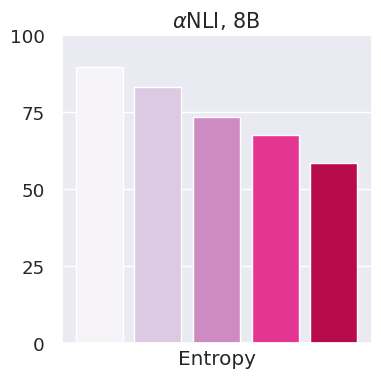
\includegraphics[height=2.2cm, trim=10 30 0 0, clip]{figures/entropy_acc_abductivenli_8B}
        \end{subfigure}
        \begin{subfigure}[b]{0.35\textwidth}
            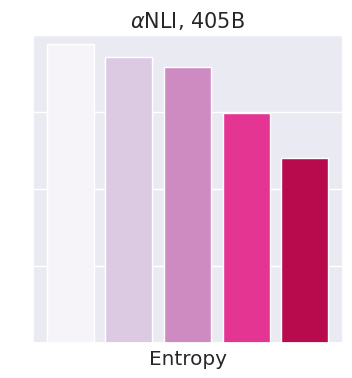
\includegraphics[height=2.2cm, trim=10 30 0 0, clip]{figures/entropy_acc_abductivenli_405B}
        \end{subfigure}\\
        \begin{subfigure}[b]{0.48\textwidth}
            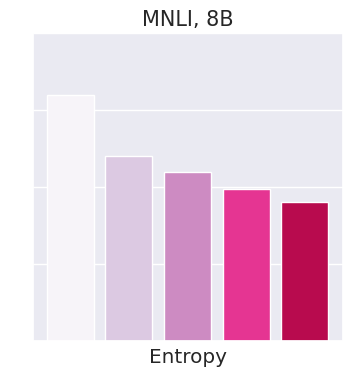
\includegraphics[height=2.2cm, trim=10 30 0 0, clip]{figures/entropy_acc_mnli_matched_8B}
        \end{subfigure}
        \begin{subfigure}[b]{0.35\textwidth}
            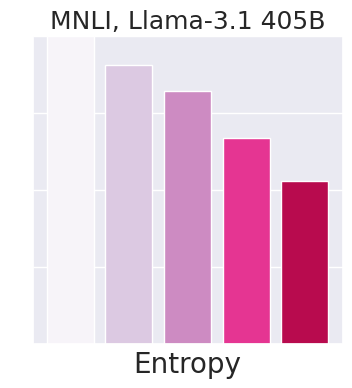
\includegraphics[height=2.2cm, trim=10 30 0 0, clip]{figures/entropy_acc_mnli_matched_405B}
        \end{subfigure}\\
        \begin{subfigure}[b]{0.48\textwidth}
            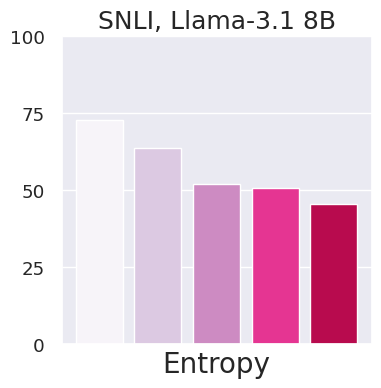
\includegraphics[height=2.4cm, trim=10 0 0 0, clip]{figures/entropy_acc_snli_8B}
        \end{subfigure}
        \begin{subfigure}[b]{0.35\textwidth}
            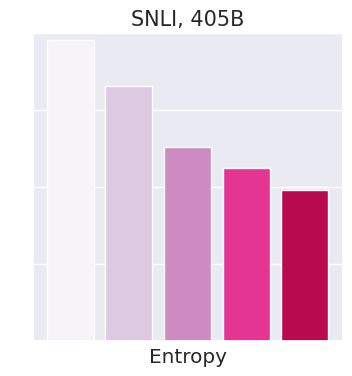
\includegraphics[height=2.4cm, trim=10 0 0 0, clip]{figures/entropy_acc_snli_405B}
        \end{subfigure}
        \caption{Accuracy vs Entropy}
         \label{fig:entropy_accuracy}
    \end{subfigure}
    \hspace{5mm}
    \begin{subfigure}[b]{0.65\textwidth}
    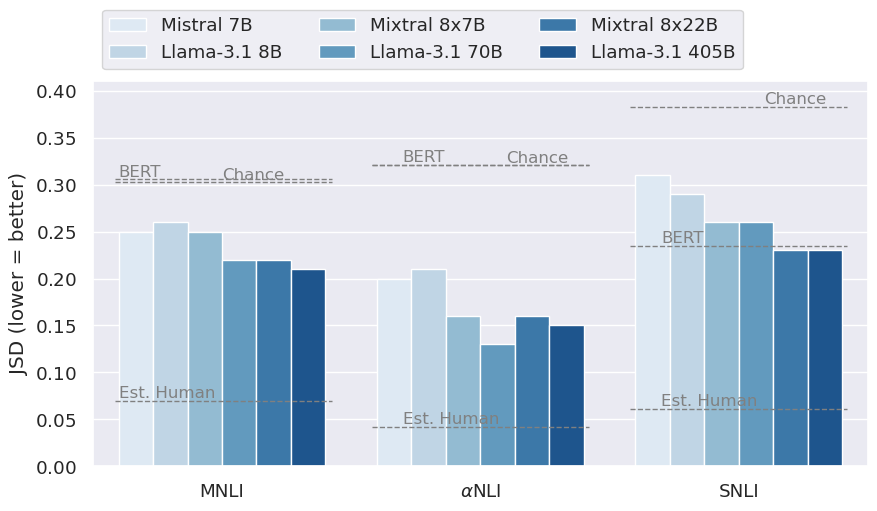
\includegraphics[width=\linewidth]{figures/jsd_all_benchmarks}
    \caption{Final model JSD}
    \label{fig:jsd_all_benchmarks}
    \end{subfigure}
    \caption{\textbf{Accuracy vs entropy and final model JSDs} 
    a) Accuracy vs entropy for Llama8B and Llama 405B. 
     We show how the accuracy of Llama 8B and Llama 405B changes as the entropy of the human label distributions increases. Accuracy-vs-entropy plots for all other models can be found in \cref{fig:entropy_accuracy_all}.
    b) Final model JSDs for each of the benchmarks in ChaosNLI. 
    JSDs are substantially lower than chance and BERT JSDs, but substantially higher than JSDs between humans.
    }
\end{figure*}

\paragraph{Implications for saturation}
What the implication of these results is for the question of saturation of these benchmarks is, like the samples of the benchmark themselves, open to interpretation.
On the one hand, it appears that for several cases, the model predictions do not align with the human majority label, suggesting that the performance may still improve as models continue training.
On the other, the results put into question whether strong alignment with the majority label is in fact what we should strive for: if humans have low agreement on their judgements, should the desired behaviour of a model be to side with the majority?
In the next section, we approach this question by considering the distribution of model outputs, rather than only the highest probability label.

% Benchmark: mnli_matched
% Number of examples: 1599
% Number of flipped labels: 508
% Number of same labels: 1091
% Percentage of flipped labels: 31.77
% 
% Benchmark: snli
% Number of examples: 1514
% Number of flipped labels: 378
% Number of same labels: 1136
% Percentage of flipped labels: 24.97
% 
% Benchmark: abductivenli
% Number of examples: 1532
% Number of flipped labels: 163
% Number of same labels: 1369
% Percentage of flipped labels: 10.64

\begin{figure*}[t]
    \centering
    \begin{subfigure}[b]{0.32\textwidth}
        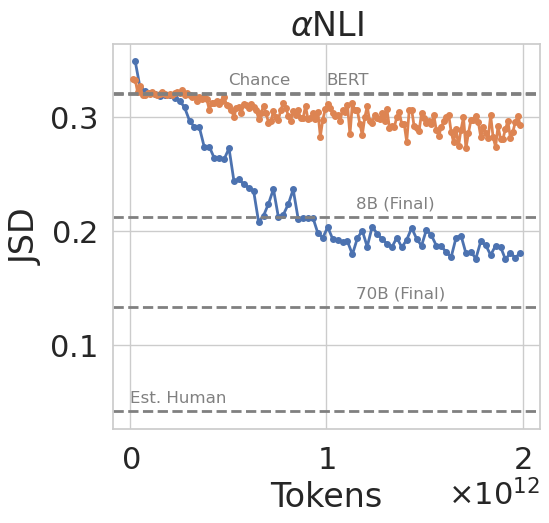
\includegraphics[height=4.5cm]{figures/abductivenli_intermediate_jsd}
        % \caption{}
    \end{subfigure}
    \begin{subfigure}[b]{0.32\textwidth}
        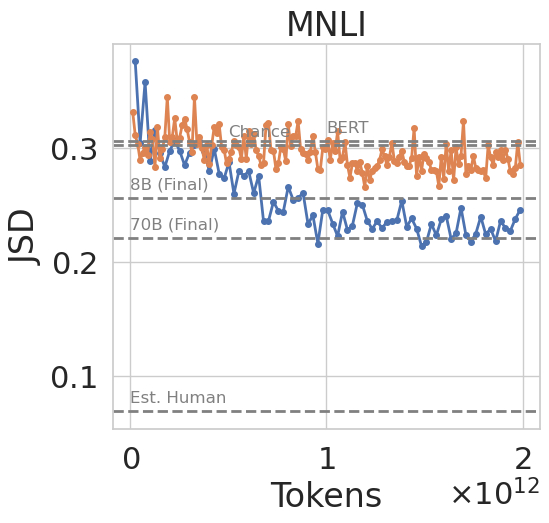
\includegraphics[height=4.5cm, trim=11mm 0 0 0, clip]{figures/mnli_matched_intermediate_jsd}
        % \caption{}
    \end{subfigure}
    \begin{subfigure}[b]{0.32\textwidth}
        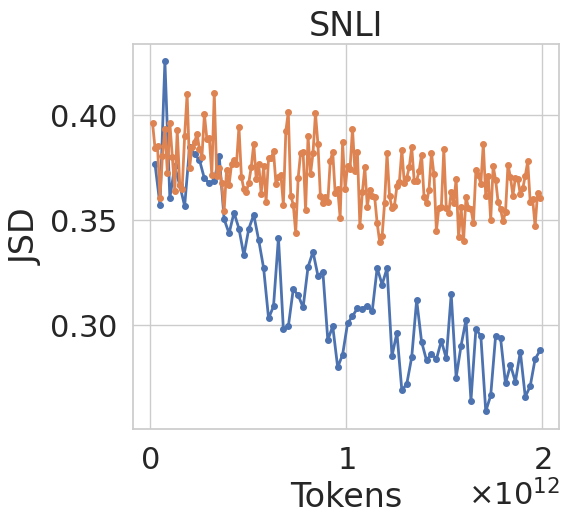
\includegraphics[height=4.5cm, trim=11mm 0 0 0, clip]{figures/snli_intermediate_jsd}
        % \caption{}
    \end{subfigure}
    \caption{\textbf{Development of JSD during training.} We show how the JSD of our trained-from-scratch 8B and 70B model develops during training.}\label{fig:jsd_training}
\end{figure*}

\subsection{Model versus human distributions}\label{subsec:chaosnli_dist}
The ChaosNLI dataset does not only help us estimate the adequacy of the original label sets of the respective datasets, but also reveals model behaviour in scenarios without a single correct answer.
In a time where LLMs are deployed for many users with potentially different preferences, this question has become very practically relevant.
To do so, we consider how the probability distribution of the models over the three possible labels \textit{Entailment}, \textit{Neutral}, and \textit{Contradiction}) compares with the label distributions observed in the human annotations.
Following \citet{nie-etal-2020-learn}, we consider Jensen-Shannon Divergence \citep[JSD][]{menendez1997jensen} to measure the distance between the two distributions. 
%Mathematically,
%
%\[
%    JSD(p || q) = \sqrt{\frac{1}{2}KL(p || m) + \frac{1}{2}KL(q || m)},
%\]
%
%where $p$ is the human annotator distribution, $q$ is the softmax probability distribution, and $m = \frac{1}{2}(p + q)$. 
Contrary to KL divergence, JSD is symmetric and bound between 0 and 1, making it more interpretable for our specific case.

In \cref{fig:jsd_all_benchmarks}, we can see that, for MNLI, all models have probability distributions more similar to the human distributions than chance, but substantially different than humans have among each other.\footnote{The human estimate was computed by \citet{nie-etal-2020-learn}, on an independent sample of human labels on the same data.}
This pattern is constant across datasets.
Interestingly, larger models have lower divergence, contradicting the finding of \citet{nie-etal-2020-learn} that better or larger models do not have more similar distributions.
Yet, the effect of scale is further confirmed in \cref{fig:jsd_training}: though even trained-out models are far away from a low JSD, the JSD of the model softmax distributions and the human label distributions decreases steadily during training.
This is an exciting finding, since it suggests that measuring similarity with human distributions could be an interesting venue to explore during training.

